\subsection{Euler-Lagrange Equation}

\subsubsection{DifferentialundefinedEquationundefinedfromundefinedPhysics}

Aundefinedlotundefinedofundefinedphysicalundefinedscienceundefinedandundefinedengineeringundefinedisundefinedaboutundefinedfindingundefinedaundefinedreductionundefinedfromundefinedaundefinedphysicalundefinedproblemundefinedtoundefineddifferentialundefinedequations.undefinedTheundefinednewtownianundefinedwayundefinedisundefinedtoundefinedzoomundefinedintoundefinedsomeundefinedlocalundefinedpointundefinedofundefinedtheundefinedsystemundefinedandundefinedderiveundefinedaundefinedsetundefinedofundefinedconstraintundefinedthatundefinedholdsundefinedinundefinedtheundefinedneighborhood.undefinedInundefinedtheundefinedcaseundefinedofundefinedtheundefinedvibrationundefinedofundefinedaundefinedstring,undefinedforundefinedexample,undefinedweundefinedwouldundefinedfindundefinedsomeundefinedlocalundefinedsegmentundefinedofundefinedstringundefinedandundefinedanalyzeundefinedtheundefinedtensionundefinedthatundefinedactsundefinedonundefinedit:
\begin{equation}
T(\sin(\theta_1)-\sin(\theta_2)) = m\frac{\partial^2 u}{\partial t^2}
\end{equation}
whereundefined$u$undefinedisundefinedtheundefinedverticalundefineddisplacementundefinedfromundefinedequilibrium.undefinedWeundefinedthenundefinedtakeundefinedtheundefinedcalculusundefinedlimitundefinedandundefinedfindundefinedoutundefinedthatundefinedlocallyundefinedtheundefinedaccelearationundefinedofundefinedtheundefinedverticalundefineddisplacementundefinedshouldundefinedbeundefinedproportionalundefinedtoundefinedtheundefinedcurvature.undefinedHenceundefinedtheundefinedone-dimensionalundefinedwaveundefinedequation:
\begin{equation}
\frac{\partial^2 u}{\partial t^2}=a^2 \frac{\partial^2 u}{\partial x^2}
\end{equation}
\footnote{Hereundefined$a$undefinedisundefinedaundefinedphysicalundefinedparameterundefinedintrinsicundefinedtoundefinedtheundefinedstring,undefinedi.e.,undefined$\sqrt{T}{\rho}$undefinedwhereundefined$T$undefinedisundefinedtheundefinedtensionundefinedatundefinedequilibriumundefinedadnundefined$\rho$undefinedisundefinedtheundefineddensity.}

TheundefinedLagrangianundefinedwayundefinedisundefinedtheundefinedopposite,undefinedweundefinedrecognizeundefinedsomeundefinedglobalundefinedobjectiveundefinedtheundefinedsystemundefinedneedundefinedtoundefinedbeundefinedoptimizedundefinedtoward,undefinedi.e.,undefinedminimizingundefinedtheundefinedlagragianundefined$L=T -V$undefinedwhereundefined$T$undefinedisundefined\textit{kineticundefinedenergy}undefinedandundefined$V$undefinedisundefined\textit{potentialundefinedenergy}.undefinedThen,undefinedbyundefinedintroduceundefinedsomeundefinedperturbation,undefinedweundefinedextractundefinedaundefinedconstraintundefinedwhichundefinedalsoundefinedmanifestundefineditselfundefinedasundefinedaundefineddifferentialundefinedequation.undefinedTheundefinedfollowingundefinedsectionsundefineddescirbesundefinedthisundefinedprocessundefinedinundefineddetail.

\begin{mystadmonition}{mystAmber}{NewtonianundefinedandundefinedLagrangianundefinedMechanics}\begin{itemize}
\item Newtonianundefinedmechanicsundefinedcomputeundefinedtheundefinedbalanceundefinedofundefinedforcesundefinedlocallyundefinedandundefinedobtainundefineddifferentialundefinedequationundefinedthroughundefined

\begin{equation}
F=m\frac{d^2\mathbf{x}}{dt^2}
\end{equation}


\item LagrangianundefinedmechanicsundefinedtranslateundefinedtheundefinedphysicsundefinedintoundefinedsomeundefinedglobalundefinedoptimizationundefinedproblemundefinedundefinedandundefinedreduceundefinedtoundefineddifferentialundefinedequationundefinedthroughundefinedtheundefinedEuler-Lagrangeundefinedequation

\begin{equation}
\frac{\partial L}{\partial y}- \frac{d}{dx}\frac{\partial L}{\partial y'}=0
\end{equation}
\end{itemize}

\end{mystadmonition}
\subsubsection{Functionalundefined:undefinedAundefinedglobalundefinedoptimizationundefinedobjective}

Aundefinedfunctionalundefinedinundefined\textit{calculusundefinedofundefinedvariation}undefinedisundefinedaundefinedmapundefinedfromundefinedaundefinedfunctionundefinedtoundefinedaundefinedrealundefinednumber,undefinedi.e.,undefined$J:C^{\infty} \to \mathbb{R}$.undefinedInundefinedparticular,undefineditundefinedmostlyundefinedcomesundefinedinundefinedsomeundefinedsortundefinedofundefinedaundefinedintegral.undefinedTheundefinedsimplestundefinedformundefinedbeingundefinedanalgousundefinedtoundefinedthatundefinedofundefinedtheundefinedlagrangian:

\begin{equation}
\label{basicfunctional}
J[y] = \int_{x_1}^{x_2} f(x,y,y')dx
\end{equation}

Theundefinedaboveundefinedexampleundefinedsufficeundefinedtoundefinedestablishundefinedtheundefinedexplictundefinedconnectionundefinedofundefined(\ref{basicfunctional})toundefinedLagrangian:

\begin{mystthmexample}{Theundefinedlagrangianundefinedforundefinedtheundefinedvibratingundefinedstring}{example-eulerlagrangeequation-1}Letundefined$u$undefinedbeundefineddeviationundefinedfromundefinedtheundefinedequilibriumundefinedposition

\begin{enumerate}
\item \textbf{Theundefinedkineticundefinedenergy}:

\begin{equation}
T=\frac{1}{2}\int_{0}^L \rho u_t(x,t)^2dx
\end{equation}


whereundefined$L$undefinedisundefinedtheundefinedlengthundefinedofundefinedtheundefinedstring


\item \textbf{Theundefinedpotentialundefinedenergy}:

\begin{equation}
V=\frac{1}{2}k\int_{0}^L {1+u_x^2} dx
\end{equation}

\footnote{Itundefinedisundefinedtemptingundefinedforundefinedsomeundefinedofundefinedusundefinedwhoundefinedareundefinednotundefinedtrainedundefinedasundefinedaundefinedphysicsundefinedstudentundefinedtoundefinedwriteundefinedtheundefinedpotentialundefinedenergyundefinedasundefined$\frac12 \left(\int_a^b \sqrt{1+u_x^2}dx\right)^2$.undefinedTheundefinedrationaleundefinedisundefinedasundefinedfollows:undefinedifundefinedweundefinedpauseundefinedatundefinedaundefinedmomentundefinedandundefinedstraigtenundefinedtheundefinedvibratingundefinedstringundefinedasundefinedaundefinedline.undefinedThenundefinedweundefinedobserveundefinedhowundefinedmuchundefinedelongationundefinedhadundefinedhappenedundefinedandundefineduseundefinedhooke'sundefinedlawundefinedonundefinedtheundefinedentireundefinedstring.undefinedThisundefinedisundefinedphysicallyundefinedwrongundefinedsinceundefinedtheundefinedelongationundefinedhappensundefinedinhomogenouslyundefinedhenceundefinedweundefinedhaveundefinedtoundefinedapplyundefinedhooke'sundefinedlawundefinedlocallyundefinedandundefinedintegrate.undefinedAlsoundefinedmathematically,
\begin{equation}
\left(\int f\right)^2 =\int f^2
\end{equation}
iffundefined$f$undefinedisundefinedsomeundefinedconstantundefinedfunction.undefinedTheundefinedgeneralundefinedrelatinoshipundefinedcanundefinedbeundefinedobtainedundefinedfromundefinedCauchy-Shwarzundefinedinequalityundefinedbyundefinedtakingundefined$f=\sqrt{1+u_x^2}$undefinedandundefined$g=1$
\begin{equation}
\left(\int_0^L \sqrt{1+u_x^2}\right)^2 \leq \int_0^L 1+u_x^2 dx
\end{equation}}
\end{enumerate}

Theundefinedlagrangianundefinedisundefinedhence:
\begin{equation}
L=\int_0^L \frac{1}{2} \left(\rho u_t(x,t)^2 - k(1+u_x^2)\right)
\end{equation}

\end{mystthmexample}
\begin{figure}[!htbp]
\centering
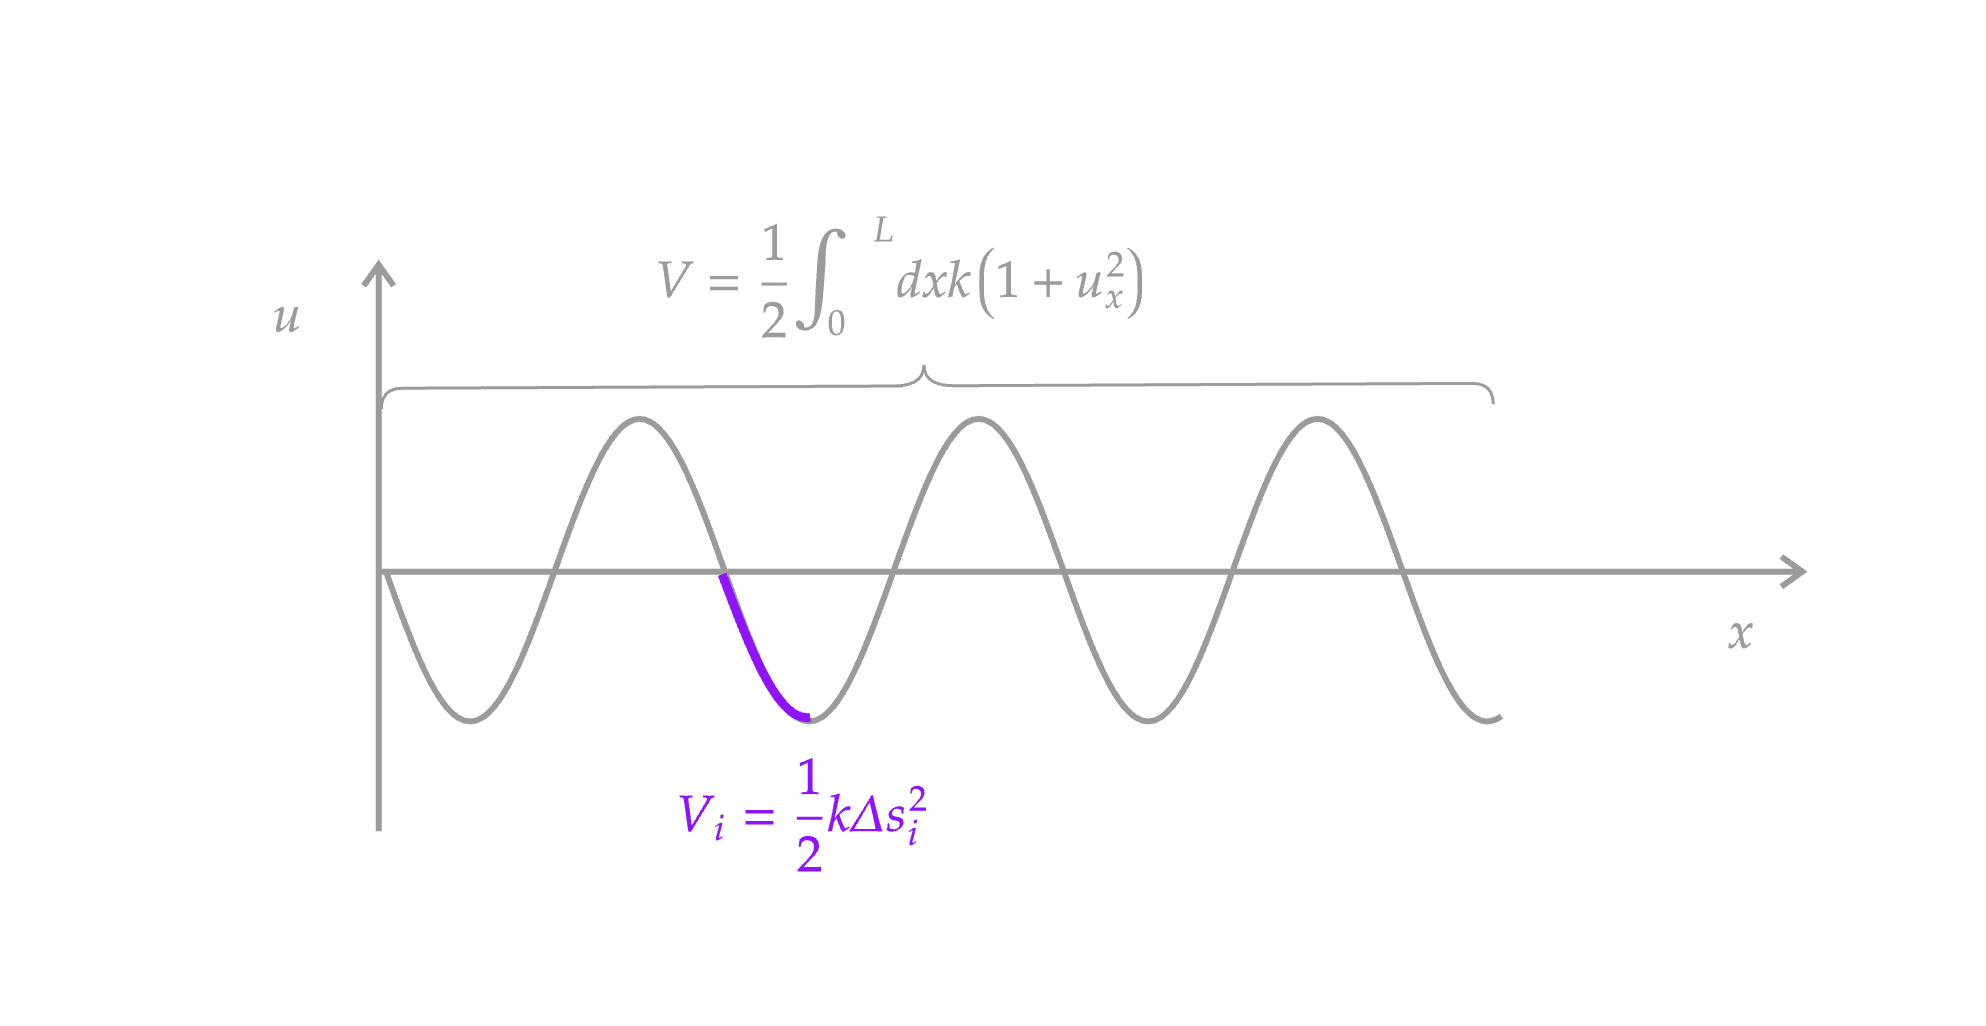
\includegraphics[width=0.7\linewidth]{files/vs-89ee0e6d488b170eecb5d0f3a41cc551.png}
\caption*{Theundefinedpotentialundefinedenergyundefinedofundefinedaundefinedvibratingundefinedstring.}
\end{figure}

Weundefinednowundefinedscrutinizeundefinedhowundefinedexactlyundefinedweundefinedoptimizeundefined(\ref{basicfunctional}).

\subsubsection{Euler-LagrangeundefinedEquation}

\begin{mystthmtheorem}{Euler-LagrangeundefinedEquation}{theorem-eulerlagrangeequation-2}$y$undefinedisundefinedaundefinedstationaryundefinedpointundefinedfor
\begin{equation}
J[y] = \int_{x_1}^{x_2} f(x,y,y^{(1)},...,y^{(n)})dx
\end{equation}
iff:
\begin{equation}
\boxed{\frac{\partial f}{\partial y} -\frac{d}{dx}\left(\frac{\partial f}{\partial y'}\right)=0}
\end{equation}
Theundefinedboxedundefinedequationundefinedisundefinedknownundefinedasundefinedtheundefined\textbf{Euler-LagrangeundefinedEquation}

\end{mystthmtheorem}
\subsubsection{DiscretizedundefinedEuler-LagrangeundefinedEquation}

\subsubsection{FirstundefinedIntegral}

\begin{mystthmdefinition}{FirstundefinedIntegral}{definition-eulerlagrangeequation-3}Suppose
\begin{equation}
y^{(n)}=f(x,y,y^{(1)},...,y^{(n-1)})
\end{equation}

isundefinedanundefinedordinaryundefineddifferentialundefinedequationundefinedofundefinedorderundefined$n$.undefinedWeundefinedcanundefineddefineundefinedanundefinedequivalentundefined$n$-dimensionalundefinedsystemundefinedbyundefinedletting:
\begin{equation}
\begin{aligned}
y_1 &= y \\
y_2 &= y^{(1)} \\
\vdots \\
y_{n} &= y^{(n-1)}
\end{aligned}
\end{equation}
Denoteundefinedby:
\begin{equation}
\frac{dy_i}{dx}=f_i(x,y_1,...,y_n)
\end{equation}
Nowundefinedsupposeundefined$f$undefinedis:

\begin{enumerate}
\item Continousundefinedaboutundefined$x,y_1,...,y_n$
\item Continuouslyundefineddifferentialbeundefinedaboutundefined$y_1,...,y_n$
\end{enumerate}

Defineundefinedundefinedtheundefined\textit{firstundefinedintegral}undefinedofundefinedtheundefined$n^{\text{th}}$-orderundefinedproblemundefinedtoundefinedbeundefinedaundefinedfunctionundefined$I=I(x,y_1,...,y_n)$undefinedthatundefinedalsoundefinedsatisfiesundefinedtheundefinedaboveundefinedtwoundefinedrequirementsundefined,undefinedandundefinedfurthermoreundefinedhasundefinedtheundefineddefinitiveundefinedproperty:
\begin{equation}
I(x,y_1,...,y_n)=\text{Constant}
\end{equation}
alongundefinedsolutionundefinedcurvesundefined$\Gamma=(y_1(x),y_2(x),...,y_n(x))$undefinedwithundefinedtheundefinedconstantundefineddeterminedundefinedbyundefinedtheundefinedsolutionundefinedcurve.

\end{mystthmdefinition}
Weundefinedareundefinedconfrontedundefinedbyundefinedtheundefinedhigher-orderundefinedordinaryundefineddifferentialundefinedequation:
\begin{equation}
\label{ele}
\frac{\partial f}{\partial y} -\frac{d}{dx}\left( \frac{\partial f}{\partial y'}\right)=0
\end{equation}
Theundefinedcomputeundefinedtheundefinedfirstundefinedintegralundefinedofundefinedthisundefinedequationundefinedisundefinedtoundefinedrewriteundefinedtheundefinedaboveundefinedtoundefinedobtainundefinedanundefinedequationundefinedofundefinedtheundefinedform:
\begin{equation}
\frac{d}{dt}I(x,y,y',...)=0
\end{equation}
Theundefinedstrategyundefinedisundefinedtoundefinedcomputeundefinedtheundefineddifferenceundefinedbetweenundefined(\ref{ele})undefinedandundefinedtheundefinedexactundefineddifferential:
\begin{equation}
\frac{df}{dx}=\frac{\partial f}{\partial x} + \sum_{j\geq 0}\frac{\partial f}{\partial y^{(j)}}\frac{dy^{(j)}}{dx}=\frac{\partial f}{\partial x} +\frac{\partial f}{\partial y}\frac{dy}{dx}+\frac{\partial f}{\partial y^{(1)}}\frac{dy^{(1)}}{dx}+\cdots
\end{equation}
Ifundefinedweundefinedmultiplyundefined(\ref{ele})undefinedbyundefined$y'$undefinedandundefinedsubtractundefinedtheundefinedtwoundefinedequationsundefinedweundefinedget:

\begin{equation}
\frac{df}{dx}-y'\left\{\frac{\partial f}{\partial y} - \frac{d}{dx}\left( \frac{\partial f}{\partial y'}\right)\right\} =\frac{\partial f}{\partial x} + \textcolor{cyan}{y''\frac{\partial f}{\partial y'}+ y'\frac{d}{dx}\left( \frac{\partial f}{\partial y'}\right)}-\sum_{j\geq 2}\frac{\partial f}{\partial y^{(j)}}\frac{dy^{(j)}}{dx}
\end{equation}

\begin{mystadmonition}{mystGreen}{Theundefinedparticularundefinedformundefinedthatundefinedallowsundefinedeasyundefinedfirstundefinedintegral}Ifundefinedweundefinedassumeundefined$f$undefinedisundefinedonlyundefineddependentundefinedonundefined$y,y'$,undefinedtheundefinedaboveundefinedbecomesundefined$f(y,y')$,undefinedthen
\begin{equation}
\begin{aligned}
\sum_{j\geq 2}\frac{\partial f}{\partial y^{(j)}}\frac{dy^{(j)}}{dx} &= 0\\ 
\frac{\partial f}{\partial x} &=0
\end{aligned}
\end{equation}

\end{mystadmonition}
Now:
\begin{equation}
\begin{aligned}
\frac{df}{dx}-\underbrace{y'\left\{\frac{\partial f}{\partial y} - \frac{d}{dx}\left( \frac{\partial f}{\partial y'}\right)\right\}}_{0}&= \frac{d}{dx}\left(y'\frac{\partial f}{\partial y'}\right)
\end{aligned}
\end{equation}
Hence:
\begin{equation}
\frac{d}{dx}\left(f-y'\frac{\partial f}{\partial y'}\right)=0
\end{equation}
Weundefinedhaveundefinedsucesfullyundefinedobtainedundefinedtheundefinedfirstundefinedinetgral:
\begin{equation}
I(y,y)=f-y'\frac{\partial f}{\partial y'}
\end{equation}

\subsubsection{Exercises}

\paragraph{Euler-LagrangeundefinedEquationundefinedforundefinedMultipleundefinedIndependentundefinedVariables}

\textbf{Prove}undefinedthat:

\begin{mystthmtheorem}{Euler-LagrangeundefinedEquation}{theorem-eulerlagrangeequation-4}Considerundefinedtheundefinedfunctional
\begin{equation}
J[y]=\int f(x_1,x_2,...,x_n,y_{x_1},y_{x_2},...,y_{x_n})d\mathbf{x}
\end{equation}
Showundefinedthatundefinedtheundefinedstationaryundefinedisundefinedacheivedundefinediff:
\begin{equation}
\frac{\partial f}{\partial y} - \sum_{i}\frac{d}{dx}\left(\frac{\partial f}{\partial y_{x_i}}\right)
\end{equation}

\end{mystthmtheorem}

\bigskip
\centerline{\rule{13cm}{0.4pt}}
\bigskip

\paragraph{Fermat'sundefinedPrincipleundefined}

\begin{mystadmonition}{mystBlue}{Note}\footnote{FromundefinedDr.undefinedP.Draper'sundefinedhomeworkundefinedproblemsundefinedforundefinedPHYSundefined508(\textit{MathematicalundefinedPhysicsundefinedI})undefinedatundefinedUIUC.}\textbf{Fermat'sundefinedPrinciple}\\
Theundefinedpathundefinedtakenundefinedbyundefinedaundefinedrayundefinedofundefinedlightundefinedbetweenundefinedanyundefinedtwoundefinedpointundefinedmakesundefinedstationaryundefinedtheundefinedtravelundefinedtimeundefinedbetweenundefinedthoseundefinedpoints.

\end{mystadmonition}
Weundefinedalsoundefineddefine:

\begin{mystthmdefinition}{RefractiveundefinedIndex}{definition-eulerlagrangeequation-5}Aundefinedmediumundefinedisundefinedcharacterizedundefinedbyundefinedtheundefinedspeedundefinedofundefinedlightundefinedtravelingundefinedthrough.undefinedSpecifically,undefinedtheundefinedrefractiveundefinedindexundefinedisundefineddefinedundefinedbyundefined$n=\frac{c}{\text{speed of light traveling in the medium}}$

\end{mystthmdefinition}
\begin{mystadmonition}{mystAmber}{\textbf{Problemundefined1}undefinedLightundefinedPropagtesundefinedinundefinedStraightundefinedLineundefinedinundefinedHomogenousundefinedMedia}\begin{enumerate}
\item \textbf{Showundefinedthatundefinedlightundefinedpropagatesundefinedalongundefinedaundefinedstragihtundefinedlineundefinedinundefinedhomogenousundefinedmedia.}
\end{enumerate}

\end{mystadmonition}
\begin{mystadmonition}{mystGreen}{\emph{Solution}}Sinceundefined$n$undefinedisundefinedindependentundefinedofundefinedpositionundefinedinundefinedhomogenousundefinedmedia,undefinedmakeundefinedstationaryundefinedtheundefinedtravelundefinedtimeundefinedisundefinedequivalentundefinedtoundefinedmakeundefinedstationaryundefinedtheundefinedlengthundefinedofundefinedtheundefinedpathundefinedtaken.undefinedNowundefinedtheundefinedproblemundefinedisundefinedequivalentundefinedtoundefinedoptimizing:
\begin{equation}
\int_{x_1}^{x_2} \sqrt{1+y'^2}dx
\end{equation}
Note:
\begin{equation}
f_y = 0 \quad f_y' = \frac{y'}{\sqrt{1+y'^2}}
\end{equation}
TheundefinedEuler-Lagrangeundefinedequationundefinedis,undefinedtherefore:
\begin{equation}
\begin{aligned}
\frac{}{}
    \frac{d}{dx}\left[ \frac{y'}{\sqrt{1+y'^2}}\right] &= 0 \\
    \frac{y'}{\sqrt{1+y'^2}} &= C_1
\end{aligned}
\end{equation}
NoteundefinedtheundefinedL.H.Sundefinedisundefinedaundefinednon-constantundefinedfunctionundefinedofundefined$y'$,undefinedhence:
\begin{equation}
y'= C_2 \Longrightarrow y=C_2x+C_3
\end{equation}

\end{mystadmonition}
\begin{mystadmonition}{mystAmber}{\textbf{Problemundefined2}undefinedSnell'sundefinedLaw}Considerundefinedtheundefinedpropagationundefinedofundefinedlightundefinedfromundefinedaundefinedflatundefinedslabundefinedofundefinedglassundefinedofundefinedrefractiveundefinedindexundefined$n_1$undefinedintoundefinedto
anotherundefinedwithundefinedrefractiveundefinedindexundefined$n_2$.undefinedByundefinedexaminingundefinedpathsundefinedthatundefinedneedundefinednotundefinedbeundefineddifferentiable
atundefinedtheundefinedflatundefinedinterface,undefinedestablishundefinedSnell'sundefinedlaw:
\begin{equation}
n_1\sin(\theta_1) = n_2\sin(\theta_2)
\end{equation}

\end{mystadmonition}
\begin{mystadmonition}{mystGreen}{\emph{Solution}}Weundefinedconsiderundefinedtheundefinedfirstundefinedpointundefinedatundefined$(x_1, 0)$,undefinedtheundefinedsecondundefinedpointundefinedatundefined$(x_2,y_2)$undefinedwhereundefined$x_1<0<x_2$.undefinedTheundefinedtimeundefinedtakenundefinedisundefinedhence:
\begin{equation}
\int_{x_1}^{x_2} \frac{1}{v(x)}\sqrt{1+y'^2}dx
\end{equation}
where:
\begin{equation}
\begin{aligned}
v(x)=
\begin{cases}
    c/n_1 &\text{if } x<0 \\
    c/n_2 &\text{if } x>0
\end{cases}
\end{aligned}
\end{equation}
TheundefinedEuler-Lagrangeundefinedequationundefinedis:
\begin{equation}
0 + \frac{d}{dx}\left( \frac{y'}{v(x)\sqrt{1+y'^2}} \right)=0
\end{equation}
Hence:
\begin{equation}
\frac{y'}{v(x)\sqrt{1+y'^2}} =C
\end{equation}
Forundefined$x<0$,undefinedweundefinedhave:
\begin{equation}
\frac{1}{v(x)}\frac{y'}{\sqrt{1+y'^2}} = \frac{n_1}{c}\sin(\theta_1) = C_1
\end{equation}
Forundefined$x>0$,undefinedweundefinedhave:
\begin{equation}
\frac{1}{v(x)}\frac{y'}{\sqrt{1+y'^2}} = \frac{n_2}{c}\sin(\theta_2) = C_2
\end{equation}
Hence:
\begin{equation}
n_1\sin(\theta_1)=n_2\sin(\theta_2)
\end{equation}
\textbf{Question:}undefinedIfundefinedweundefinedflipundefinedtheundefinedaxisundefinedweundefinedwouldundefinedgetundefined$n_1\cos\theta_1=n_2\cos\theta_2$,undefinedwhyundefinedisundefinedthatundefinedwrong?

\end{mystadmonition}
\begin{mystadmonition}{mystAmber}{\textbf{Problemundefined3}undefinedGeneralundefinedSnell'sundefinedlaw}Aundefinedplanarundefinedlightundefinedrayundefinedpropagatesundefinedinundefinedanundefinedlayeredundefinedmediumundefinedwithundefinedrefractiveundefinedindexundefined$n(x)$.undefinedUseundefinedFermat'sundefinedprincipleundefinedtoundefinedestablishundefinedaundefinedgeneralizedundefinedSnell'sundefinedlaw:
\begin{equation}
n(x)\sin(\psi(x))=\text{constant}
\end{equation}
byundefinedfindingundefinedtheundefinedequationundefinedforundefinedstationaryundefinedpathsundefinedfor
\begin{equation}
F_1=\int n(x)\sqrt{1+y'^2}dx
\end{equation}
(Hereundefinedtheundefinedprimeundefineddenotesundefineddifferentiationundefinedwithundefinedrespectundefinedtoundefinedx.)undefinedRepeatundefinedthisundefinedexerciseundefinedwithundefined$x,y$undefinedswappedundefinedbyundefinedfindingundefinedaundefinedsimilarundefinedequationundefinedforundefinedtheundefinedstationaryundefinedpathsundefinedof
\begin{equation}
F_2=\int n(y)\sqrt{1+y'^2}dx
\end{equation}
Byundefinedusingundefinedsuitableundefineddefinitionsundefinedofundefinedtheundefinedangleundefinedofundefinedincidenceundefined$\psi$,undefinedinundefinedeachundefinedcaseundefinedshowundefinedthatundefinedtheundefinedtwoundefinedformulationsundefinedofundefinedtheundefinedproblemundefinedofundefinedaundefinedlayeredundefinedmediumundefinedgiveundefinedphysicallyundefinedequivalentundefinedanswers.
(Inundefinedtheundefinedsecondundefinedformulationundefinedyouundefinedwillundefinedfindundefineditundefinedeasiestundefinedtoundefineduseundefinedtheundefinedfirstundefinedintegral.)

\end{mystadmonition}
\paragraph{DrumsundefinedandundefinedMembranesundefined}

\footnote{FromundefinedDr.undefinedP.Draper'sundefinedhomeworkundefinedproblemsundefinedforundefinedPHYSundefined508(\textit{MathematicalundefinedPhysicsundefinedI})undefinedatundefinedUIUC.}Theundefinedshapeundefinedofundefinedaundefineddistortedundefineddrumskinundefinedisundefineddescribedundefinedbyundefinedthe
functionundefined$h(x, y)$,undefinedwhichundefinedgivesundefinedtheundefinedheightundefinedtoundefinedwhichundefinedtheundefinedpointundefined$(x, y)$undefinedofundefinedtheundefinedflatundefinedundistortedundefineddrumskinundefinedisundefineddisplaced.

\begin{mystadmonition}{mystAmber}{\textbf{Problemundefined1}undefinedAreaundefinedofundefineddistortedundefineddrumskin}Showundefinedthatundefinedtheundefinedareaundefinedofundefinedtheundefineddistortedundefineddrumskinundefinedisundefinedequalundefinedto
\begin{equation}
A[h] = \int dxdy \sqrt{1 + \partial_x h^2 + \partial_y h^2}
\end{equation}

\end{mystadmonition}
\begin{mystadmonition}{mystGreen}{\emph{Solution}}Considerundefinedtheundefinedareaundefineddifferntialundefined$dA=ds_x ds_y$undefinedwhereundefined$ds_x=\sqrt{1+\partial_x h^2}dx$undefinedandundefined$ds_y=\sqrt{1+\partial_y h^2}dy$undefinedhence
\begin{equation}
dA=\sqrt{1+\partial_x h^2 + \partial_y h^2 + (\partial_x h\partial_y h)^2}dxdy
\end{equation}
sinceundefined$\partial_x h\partial_y h\in \mathcal{O}(d\rho^2)$undefinedwhereundefined$d\rho = \sqrt{dx^2 + dy^2}$undefinedweundefinedcanundefineddropundefinedit.undefinedAsundefineddesired.

\end{mystadmonition}
\begin{mystadmonition}{mystAmber}{Areaundefinedforundefinedsmallundefineddistortion}Showundefinedthatundefinedforundefinedsmallundefineddistortions,undefinedtheundefinedareaundefinedreducesundefinedto
\begin{equation}
\label{afsd}
   A[h]=\frac{1}{2}\int dxdy |\nabla h|^2 + \text{constant}
\end{equation}

\end{mystadmonition}
\begin{mystadmonition}{mystGreen}{\emph{Solution}}Recallundefinedtheundefinedgeneralizedundefinedbinomialundefinedtheorem:
\begin{equation}
(1+x)^{\alpha}=1+\alpha x + \frac{\alpha(\alpha-1)}{2!}x^2+\cdots + \frac{\alpha(\alpha-1)...(\alpha-n+1)}{n!}x^n + \cdots
\end{equation}
forundefined$|x|<1$.
Asundefinedaundefinedresult:
\begin{equation}
(1+x)^{1/2}=1+\frac12 x + \mathcal{O}(x^2)
\end{equation}
Assumeundefinedaundefinedsmallundefinedperturbation,undefinedinundefinedparticular,undefinedassumeundefined$|\nabla h|^2 \ll 1$,undefinedthen
\begin{equation}
\sqrt{1+|\nabla h|^2} = 1 + \frac12 |\nabla h|^2 +  \mathcal{O}(|\nabla h|^4)
\end{equation}
Asundefinedaundefinedresult,
\begin{equation}
A[h]=\frac12 \int dxdy |\nabla h|^2 + \underbrace{\int dxdy}_{\text{constant}}
\end{equation}

\end{mystadmonition}
\begin{mystadmonition}{mystAmber}{\textbf{Problemundefined3}}Showundefinedthatundefinedifundefined$h$undefinedsatisfiesundefinedtheundefinedtwo-dimensionalundefinedLaplaceundefinedequationundefinedthenundefined$A$undefinedisundefinedstationaryundefinedwith
respectundefinedtoundefinedvariationsundefinedthatundefinedvanishundefinedatundefinedtheundefinedboundary.

\end{mystadmonition}
\begin{mystadmonition}{mystGreen}{\emph{Solution}}WeundefinedneedundefinedthatundefinedtheundefinedEuler-Lagrangeundefinedequationundefinedforundefined(\ref{afsd})undefinedisundefinedequivlanetundefinedtoundefinedtheundefinedtow-dimensionalundefinedLaplaceundefinedequation.undefinedThatundefinedisundefinedsimple:undefinedletundefined$f(x,y,h, h_x,h_y)=h_x^2 + h_y^2$,
\begin{equation}
\begin{aligned}
\frac{\partial f}{\partial h} + \frac{d}{dx}\left(\frac{\partial f}{\partial h_x}\right) + \frac{d}{dy}\left(\frac{\partial f}{\partial h_y}\right) &= 0 \\
 0 + 2\left(\frac{dh_x}{dx} +  \frac{dh_x}{dx}\right) &= 0\\
 \nabla^2 h &=0
\end{aligned}
\end{equation}

\end{mystadmonition}
\begin{mystadmonition}{mystAmber}{\textbf{Problemundefined4}}Supposeundefinedtheundefineddrumskinundefinedhasundefinedmassundefined$\rho_0$undefinedperundefinedunitundefinedarea,undefinedandundefinedsurfaceundefinedtensionundefined$T$.undefinedWriteundefineddown
theundefinedLagrangianundefinedcontrollingundefinedtheundefinedmotionundefinedofundefinedtheundefineddrumskinundefinedandundefinedderiveundefinedtheundefinedequationundefinedof
motionundefinedthatundefinedfollowsundefinedfromundefinedit.

\end{mystadmonition}
\begin{mystadmonition}{mystGreen}{\emph{Solution}}Theundefinedkineticundefinedtermundefinedisundefinedgivenundefinedby:
\begin{equation}
T=\frac12 \int_{\Omega} dxdy \rho_0h_t^2
\end{equation}

Theundefinedpotentialundefinedtermundefinedis:undefined\footnote{Theundefinedkeyundefinedtoundefinedsolveundefinedthisundefinedproblemundefinedisundefinedactuallyundefinedtoundefinedrealizeundefinedthatundefinedsurfaceundefinedtensionundefinedhasundefinedtheundefineddimensionundefined$[F]/[L]=[E]/[L]^2$,undefinedinundefinedotherword,undefinedsurfaceundefinedtensionundefinedisundefinedpreciselyundefinedtheundefinedperunitundefinedpotentialundefinedenergyundefineddueundefinedtoundefined``stretching''/``distorsion''undefinedbyundefinedconstruction.}
\begin{equation}
V=\int_{\Omega} dxdy T|\nabla h|^2
\end{equation}

Henceundefinedtheundefinedlagrangianundefinedis:
\begin{equation}
\begin{aligned}
L &= T-V \\
&= \int_{\Omega} dxdy \left\{\frac12 \rho_0h_t^2 - T|\nabla h|^2 \right\}
\end{aligned}
\end{equation}

Computingundefinedtheundefinedvariousundefinedderivatives:
\begin{equation}
\frac{\partial L}{\partial h}=0 \quad \frac{\partial L}{\partial h_t}=\rho_0 h_t \quad \frac{\partial L}{\partial h_x}=-2Th_{x} \quad \frac{\partial L}{\partial h_y}=-2Th_{y}
\end{equation}

\end{mystadmonition}